\documentclass[hangout,aspectratio=1610,10pt]{beamer}
%
% Choose how your presentation looks.
%
% For more themes, color themes and font themes, see:
% http://deic.uab.es/~iblanes/beamer_gallery/index_by_theme.html
%
\mode<presentation>
{
  \usetheme{NYU}      % or try Darmstadt, Madrid, Warsaw, ...
  \usecolortheme{default} % or try albatross, beaver, crane, ...
  \usefonttheme{default}  % or try serif, structurebold, ...
  \setbeamertemplate{navigation symbols}{}
  \setbeamertemplate{caption}[numbered]
} 

\usepackage{standalone}
\usepackage[english]{babel}
\usepackage[utf8x]{inputenc}
\usepackage{multirow}
\usepackage{booktabs, tabularx, colortbl}
\usepackage{changepage}
\usepackage[noplaybutton]{media9}
\usepackage[percent]{overpic}
\usepackage{hyperref}
\usepackage{attachfile2}
\usepackage{calc}
%\usepackage{subfig}
\usefonttheme[onlymath]{serif}
\usepackage{amssymb}% http://ctan.org/pkg/amssymb
\usepackage{pifont}% http://ctan.org/pkg/pifont
\newcommand{\cmark}{\ding{51}}%
\newcommand{\xmark}{\ding{55}}%
\usepackage{graphicx}
\usepackage{subcaption}
\usepackage{svg}
\usepackage{tikz}
\usepackage{bm,physics}
\usepackage{pgfplotstable}
\usetikzlibrary{tikzmark,calc,trees}
\usetikzlibrary{decorations.markings}
\usetikzlibrary{math}
\usetikzlibrary{intersections}
\usetikzlibrary{through}
\usetikzlibrary{decorations.pathreplacing,calc,decorations.markings}
\usetikzlibrary{decorations.text}
\usetikzlibrary{backgrounds}
\usepackage{color,array}
\makeatletter
\def\zapcolorreset{\let\reset@color\relax\ignorespaces}
\def\colorrows#1{\noalign{\aftergroup\zapcolorreset#1}\ignorespaces}
\makeatother
\usepackage{centernot}

\newenvironment{variableblock}[3]{%
  \setbeamercolor{block body}{#2}
  \setbeamercolor{block title}{#3}
  \begin{block}{#1}}{\end{block}}

\newenvironment{redblock}[1]{%
  \begin{variableblock}{#1}{bg=red!20,fg=black}{bg=red!80,fg=white}}{\end{variableblock}}
\newenvironment{greenblock}[1]{%
  \begin{variableblock}{#1}{bg=green!20,fg=black}{bg=green,fg=white}}{\end{variableblock}}

\newenvironment{blueblock}[1]{%
  \begin{variableblock}{#1}{bg=blue!20,fg=black}{bg=blue,fg=white}}{\end{variableblock}}
\newenvironment{yellowblock}[1]{%
  \begin{variableblock}{#1}{bg=yellow!20,fg=black}{bg=yellow,fg=white}}{\end{variableblock}}



\newenvironment{thm}[1][Theorem]{%
    \begin{variableblock}{#1}{bg=lightblue!20,fg=black}{bg=lightblue,fg=white}}{\end{variableblock}}
\newenvironment{lem}[1][Lemma]{%
    \begin{variableblock}{#1}{bg=lightblue!20,fg=black}{bg=lightblue,fg=white}}{\end{variableblock}}
\newenvironment{prop}[1][Proposition]{%
    \begin{variableblock}{#1}{bg=blue!20,fg=black}{bg=blue,fg=white}}{\end{variableblock}}
\newenvironment{defi}[1][Definition]{%
    \begin{variableblock}{#1}{bg=purple!20,fg=black}{bg=purple,fg=white}}{\end{variableblock}}
\newcommand{\bs}[1]{\textbf{#1}}
\renewcommand{\div}[1]{\text{div}{#1}}

\newcommand{\Lchild}{\mathcal{L}^{\text{child}}}
\newcommand{\Lnei}{\mathcal{L}^{\text{nei}}}
\newcommand{\Lint}{\mathcal{L}^{\text{int}}}
\newcommand{\qhat}{\hat{\vb q}}
\newcommand{\uhat}{\hat{\vb u}}
\newcommand{\q}{\vb{q}}
\newcommand{\A}{\vb{A}}
\newcommand{\Tofs}{\vb{T}^{\text{ofs}}}
\newcommand{\Tofo}{\vb{T}^{\text{ofo}}}
\newcommand{\Tifo}{\vb{T}^{\text{ifo}}}
\newcommand{\Tifi}{\vb{T}^{\text{ifi}}}
\newcommand{\Ttfi}{\vb{T}^{\text{tfi}}}
\newcommand{\CC}{\mathbb{C}}
\usepackage{forest}
\forestset{
  % Two node styles for game trees: solid and hollow
  solid node/.style={circle,draw,inner sep=1.2,fill=black},
  hollow node/.style={circle,draw,inner sep=1.2},
  % styles for long branch labels
  left label/.style={above left,midway},
  right label/.style={above right,midway},
  arrow edges/.style = for tree={{edge={<->}}},
  qtree/.style={
  align=center,}
}
\title[Implementation of the fast multipole method]{Implementation of the fast multipole method}
\author{Shanyin Tong\quad Yu-hsuan Shih}
\institute{Courant Institute of Mathematical Sciences, New York University}
\date{12/09/2020}
\titlegraphic{\hfill
\includegraphics[height=1.5cm]{nyu_stacked_color}}


\begin{document}

\begin{frame}
  \titlepage
\end{frame}

% Uncomment these lines for an automatically generated outline.
%\begin{frame}{Outline}
%  \tableofcontents
%\end{frame}
\begin{frame}{Problem formulation}
Consider evaluating all pairwise interactions between a given set of $N$ electrically charged particles in two dimensions.
\begin{equation}
    \label{eq:sum}
    u_i =\sum_{j=1}^N G(\bm x_i,\bm x_j)q_j, \quad i =1,2,\ldots,N,
\end{equation}
$\{\bm x_i\}^N_{i=1}$: a given set of point locations in a square $\Omega$ \\
$\{q_i\}^N_{i=1}$: a given set of corresponding sources\\
$\{u_i\}^N_{i=1}$: a set of potential values to be determined\\
$G(\bm x, \bm y) = \log(\bm x - \bm y)$: kernel\\
Using $\A(i,j)=G(\bm x_i,\bm x_j), \q(i)=q_i$ and $\vb u(i)=u_i$, 
write \eqref{eq:sum} as a matrix vector multiplication: 
\begin{equation*}
    \vb u=\A \q
\end{equation*}
However, direct evaluation cost is $O(N^2)$. 
\end{frame}

\begin{frame}{Review of FMM}
To evaluate \eqref{eq:sum} in linear complexity, the fast multipole method (FMM) uses a multilevel technique, splitting the computational domain $\Omega$ into a tree of boxes. Denote the level to be $l=0,1,\ldots,L-1$, $l=0$ denotes the root and $l=L-1$ denotes the leaf boxes. Given a box $\tau$ in the hierarchical tree, define the index vectors for box $\tau$:
\begin{itemize}
    \item \textbf{parent}: the box on the next coarsest level that contains $\tau$.
    \item \textbf{children list $\Lchild_\tau$}: the set contains the boxes whose parent is $\tau$.
\item \textbf{neighbor list $\Lnei_\tau$}: the set contains the boxes on the same level that directly touch $\tau$ 
\item \textbf{interaction list $\Lint_\tau$}: the set contains all boxes $\sigma$ such that (1) $\sigma$ and $\tau$ are on the same level, (2) $\sigma$ and $\tau$ do not touch, and (3) the parents of $\sigma$ and $\tau$ do touch.
\end{itemize}
\begin{center}
    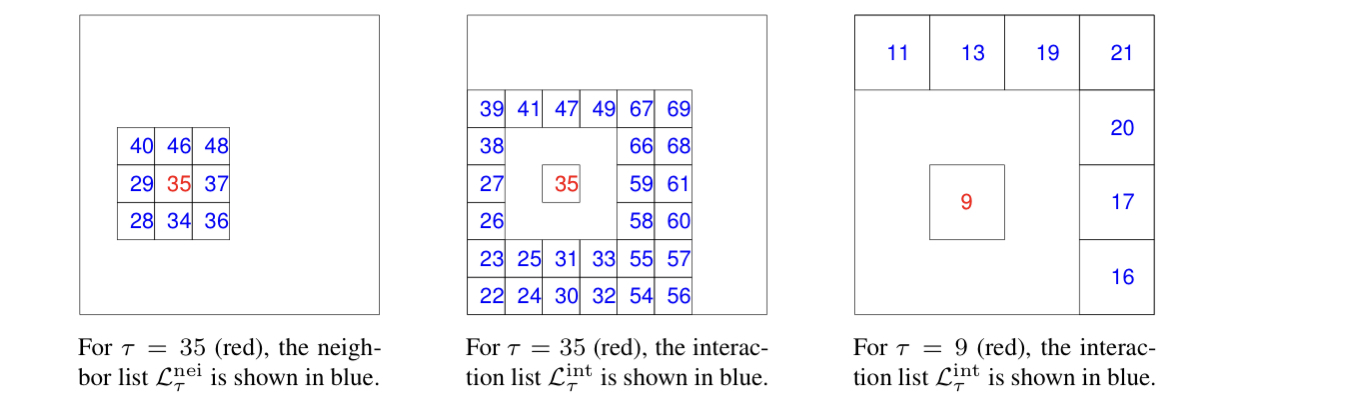
\includegraphics[width=1.\linewidth]{plots/list.jpeg}
\end{center}

\end{frame}
\begin{frame}{Review of FMM}
    Evaluating multipole expansions hierarchically. 
    \begin{itemize}
        \item \textbf{Upward pass}: Compute the outgoing expansion of each box in a pass over all boxes, going from smaller boxes to larger ones. 
        \begin{itemize}
            \item For a leaf box, compute the expansion directly from the sources in the box: $\qhat_\tau = \Tofs_\tau\; \q(I_\tau)$
            \item For a parent box, use the outgoing expansions of its children: $\qhat_\tau = \sum_{\sigma\in \Lchild_\tau} \Tofo_{\tau, \sigma}\;\qhat_\sigma$
        \end{itemize}
        \item \textbf{Downward pass}: Compute the incoming expansion for every box in a pass over all boxes, going from larger boxes to smaller ones. For each box, combine the incoming expansion of its parent $\nu$ with the contributions from the outgoing expansions of all boxes in its interaction list:\[\uhat_\tau=\Tifi_{\tau,\nu}\;\uhat_\nu+\sum_{\sigma\in\Lint_\tau}\Tifo_{\tau,\sigma}\;\qhat_\sigma\]
        \item Compute the potential on every leaf by expanding its incoming potential and then adding the contributions from its near field via direct evaluation:
        \[\vb u(I_\tau)=\Ttfi_\tau \; \uhat_\tau +\A(I_\tau,I_\tau)\; \q(I_\tau) +
\sum_{\sigma\in \Lnei_\tau}\A(I_\tau,I_\sigma)\; \q(I_\sigma)\]
    \end{itemize}
Transition operator $\Tofo_{\tau,\sigma},  \Tifo_{\tau,\sigma},\Tifi_{\tau,\sigma}\in\CC^{P\times P}$ are independent of $\{\bm x_i\}^N_{i=1}$. $\Tofs_\tau\in \CC^{P\times N_\tau}$ and $\Ttfi_\tau\in\CC^{N_\tau\times P}$ are computed for each leaf box $\tau$.
\end{frame}

\begin{frame}{Implementation}
\only<1>{
\vspace{0.5cm}
\begin{figure}
\centering
\scalebox{0.8}{
\begin{forest}
    nonterminal/.style={
        symbol,
        rounded corners,
    },
[{$B_0$} ,for tree={s sep=.3in},name=R,red,
  [{$B_{1}^{TL}$} ,name=P1,green,
    [{$B_{2}^{TL}$} ,name=P,orange,
        [{$B_{3}^{TL}$},name=c1,blue ]
        [{$B_{3}^{TR}$},name=c2,blue ]
        [{$B_{3}^{BL}$},name=c3,blue ]
        [{$B_{3}^{BR}$},name=c4,blue ]
    ]
    []
    []
    []
        %   [ ,label={below:\payoff{1\\-1}},edge label={node[left,midway] {L}} ]
        %   [ ,label={below:\payoff{0\\0}},edge label={node[right,midway] {R}} ]
        %   [ ,label={below:\payoff{1\\-1}},edge label={node[left,midway] {L}} ]
        %   [ ,label={below:\payoff{0\\0}},edge label={node[right,midway] {R}} ]]
  ]
  [{$B_{1}^{TR}$},green,
        [ ]
        [ ]
        [ ]
        [ ]
  ]
  [{$B_{1}^{BL}$},green
    [ ]
    [,no edge, edge label={node[midway] {$\dots$}}]
  ]
  [{$B_{1}^{BR}$},green]
]
\draw [<->, thick] (P) -- (c1);
\draw [<->, thick] (P) -- (c2);
\draw [<->, thick] (P) -- (c3);
\draw [<->, thick] (P) -- (c4);
\draw [<->, thick] (P) -- (P1);
\draw [<->, thick] (P1) -- (R);
\draw [->, thick, dashed] (c1) -- (c2);
\draw [->, thick,  dashed] (c2) -- (c3);
\draw [->, thick,  dashed] (c3) -- (c4);
\draw [->, thick,  dashed] (c4) to [out=200, in=-20] (c1);
\end{forest}
}
\label{fig:tree}
\caption{Diagram of the quadtree data structure. L=4.}
\end{figure}
}
\only<2->{
\vspace{0.5cm}
\begin{figure}
\centering
\scalebox{0.8}{
\begin{forest}
    nonterminal/.style={
        symbol,
        rounded corners,
        align=center,
    },
[{$B_0$} ,for tree={s sep=.3in},name=R
  [{$B_{1}^{TL}$} ,name=P
    [{$B_{2}^{TL}$},name=c1,draw,blue]
    [{$B_{2}^{TR}$},name=c2,draw,red ]
    [{$B_{2}^{BL}$},name=c3,draw,blue ]
    [{$B_{2}^{BR}$},name=c4,draw,blue ]
  ]
  [{$B_{1}^{TR}$} , name=P2
    [{$B_{2}^{TL}$},name=c21,draw,blue ]
    [{$B_{2}^{TR}$},name=c22 ]
    [{$B_{2}^{BL}$},name=c23,draw,blue ]
    [{$B_{2}^{BR}$},name=c24 ]
  ]
  [{$\dots$}]
  [{$\dots$}]
]
% \draw [<->, thick] (P) -- (c1);
% \draw [<->, thick] (P) -- (c2);
% \draw [<->, thick] (P) -- (c3);
% \draw [<->, thick] (P) -- (c4);
% \draw [<->, thick] (P) -- (R);
% \draw [<->, thick] (P2) -- (c21);
% \draw [<->, thick] (P2) -- (c22);
% \draw [<->, thick] (P2) -- (c23);
% \draw [<->, thick] (P2) -- (c24);
% \draw [<->, thick] (P2) -- (R);
\draw [->,thick,blue] (c2) -- (c1) node [midway, below] {\footnotesize\textbf{next}};
\draw [->,thick,blue] (c1) to [out=-40, in=220] (c3);
\draw [->,thick,blue] (c3) -- (c4);
\draw [->,thick,blue] (c4) -- (c21);
\draw [->,thick,blue] (c21) to [out=-30, in=200] (c23);
\end{forest}
}
\label{fig:tree}
\caption{Linked list data structure for neighbor list for the red node (box).}
\end{figure}
}
\begin{columns}
\begin{column}{0.3\textwidth}
\only<1>
{
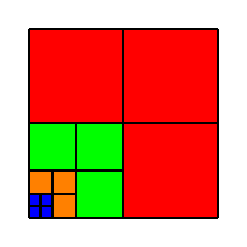
\begin{tikzpicture}[scale=0.3]
\fill[red] (4,0) rectangle (8,8);
\fill[red] (0,4) rectangle (4,8);
\fill[green] (2,0) rectangle (4,4);
\fill[green] (0,2) rectangle (2,4);
\fill[orange] (1,0) rectangle (2,2);
\fill[orange] (0,1) rectangle (1,2);
\fill[blue] (0,0) rectangle (1,1);
\draw[step=4cm, black, thick] (0,0) grid (8,8);
\draw[step=2cm, black, thick] (0,0) grid (4,4);
\draw[step=1cm, black, thick] (0,0) grid (2,2);
\draw[step=0.5cm, black, thick] (0,0) grid (1,1);
\end{tikzpicture}
}
\only<2->
{
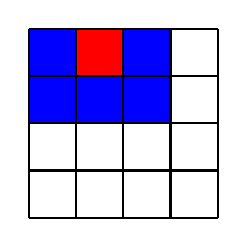
\begin{tikzpicture}[scale=0.3]
% \fill[red] (4,0) rectangle (8,8);
% \fill[red] (0,4) rectangle (4,8);
% \fill[green] (2,0) rectangle (4,4);
% \fill[green] (0,2) rectangle (2,4);
% \fill[brown] (1,0) rectangle (2,2);
% \fill[brown] (0,1) rectangle (1,2);
\fill[blue] (0,4) rectangle (6,8);
\fill[red] (2,6) rectangle (4,8);
% \draw[step=4cm, black, thick] (0,0) grid (8,8);
% \draw[step=2cm, black, thick] (0,0) grid (4,4);
\draw[step=2cm, black, thick] (0,0) grid (8,8);
\end{tikzpicture}
}
\end{column}
\begin{column}{0.7\textwidth}
\begin{itemize}
\item Step 1: Build quadtree data structure.
\pause \item Step 2: Build the parent, child, neighbor, interaction list
\pause \item Step 3: Build the translation operators $\Tofo_{\tau,\sigma}, \Tifo_{\tau,\sigma}, \Tifi_{\tau,\sigma}$.
\pause \item Step 4: Sort the particles into leaf boxes.
\pause \item Step 5: Calculate the potential using FMM.
\end{itemize}
\end{column}
\end{columns}
\end{frame}
\begin{frame}{Numerical Results}
\alert{Set up}
\begin{itemize}
\item Uniformly distributed particles. $\bs x_i$ are i.i.d. uniform random in $[0,1]^2$.
\item Given $\varepsilon$, the length of the outgoing expansion length $P$ is chosen such that 
\begin{equation*}
    \label{eq:P}
    \varepsilon\sim\eta_{\text{2D}}^P, \quad \eta_{\text{2D}}=\frac{\sqrt{2}}{4-\sqrt{2}}.
\end{equation*}
\item The depth of the tree $L$ is chosen such that each box contains roughly $P$ number of particles, \begin{equation*}
    4^{L-1} \approx N/P
\end{equation*}
\end{itemize}
\end{frame}
\begin{frame}{Accuracy tests}
\begin{figure}[ht] 
  \centering
  \pgfplotsset{filter discard warning=false}  % alex added to kill huge slow msgs

\definecolor{col-1e-3}{RGB}{0,0,255} % oranged red
\definecolor{col-1e-8}{RGB}{255,30,0} % dodgerblue
\definecolor{col-1e-13}{RGB}{0,100,50}
\definecolor{col-orange}{RGB}{255, 122, 0}
\pgfplotsset{
    discard if not/.style 2 args={
        x filter/.append code={
            \edef\tempa{\thisrow{#1}}
            \edef\tempb{#2}
            % \edef\tempc{\thisrow{#3}}
            % \edef\tempd{#4}
            \ifx\tempa\tempb
                % \ifx\tempc\tempd
                % \else
                %     \def\pgfmathresult{inf}
                % \fi
            \else
                \def\pgfmathresult{inf}
            \fi
        }
    }
}
\pgfplotsset{
    discard if/.style 2 args={
        x filter/.append code={
            \edef\tempa{\thisrow{#1}}
            \edef\tempb{#2}
            \ifx\tempa\tempb
                \def\pgfmathresult{inf}
            \else

            \fi
        }
    }
}
\hfill
\begin{tikzpicture}[
  scale=0.8,
  every axis/.style={
    xlabel={$P$},,
    log basis x={2},
    grid,
    ymin=0,
	title={},
	ylabel={relative error $\varepsilon = \| u - \tilde{u}\|_2/\|u\|_2$},
  },
]
\begin{semilogyaxis}[title={N=5000},legend pos=north west,legend cell align=left]
\addplot +[teal,mark=*,thick,mark options={fill=teal}]
           table [x=P,y=err]{data/acc.txt};
\end{semilogyaxis}
\end{tikzpicture}
\hfill
  \label{fig:fmm}
\end{figure} 
\begin{itemize}
    \item The calculated $P$ is larger than needed, e.g. for $\varepsilon=10^{-4}$, $P=15$.
\end{itemize}
\end{frame}
\begin{frame}{Performance tests}
\only<1>{
\begin{figure}[ht] 
  \centering
  % 4 plots
\pgfplotsset{filter discard warning=false}  % alex added to kill huge slow msgs

\definecolor{col-1e-3}{RGB}{0,0,255} % oranged red
\definecolor{col-1e-8}{RGB}{255,30,0} % dodgerblue
\definecolor{col-1e-13}{RGB}{0,100,50}
\definecolor{col-orange}{RGB}{255, 122, 0}
\pgfplotsset{
    discard if not/.style 2 args={
        x filter/.append code={
            \edef\tempa{\thisrow{#1}}
            \edef\tempb{#2}
            % \edef\tempc{\thisrow{#3}}
            % \edef\tempd{#4}
            \ifx\tempa\tempb
                % \ifx\tempc\tempd
                % \else
                %     \def\pgfmathresult{inf}
                % \fi
            \else
                \def\pgfmathresult{inf}
            \fi
        }
    }
}
\pgfplotsset{
    discard if/.style 2 args={
        x filter/.append code={
            \edef\tempa{\thisrow{#1}}
            \edef\tempb{#2}
            \ifx\tempa\tempb
                \def\pgfmathresult{inf}
            \else

            \fi
        }
    }
}

\hfill
\begin{tikzpicture}[
  scale=0.8,
  every axis/.style={
    xlabel={$N$ $\rightarrow$},,
    log basis x={10},
    grid,
    ymin=0,
	title={},
	ylabel=wall time (sec) $\rightarrow$,
  },
]
\begin{loglogaxis}[title={Direct v.s. FMM},legend pos=south east,legend cell align=left]
\addplot +[black, 
           mark=*,thick]
           table [x=N,y expr={(\thisrow{fmm})/1e3}]{data/dirfmm.dat};
           \addlegendentry{Direct}
\addplot +[purple, 
           mark=square*,thick]
           table [x=N,y expr={(\thisrow{dir})/1e3}]{data/dirfmm.dat};
           \addlegendentry{FMM}
\end{loglogaxis}
\end{tikzpicture}
\hfill
\begin{tikzpicture}[
  scale=0.8,
  every axis/.style={
    xlabel={$N$ $\rightarrow$},,
    log basis x={10},
    grid,
    ymin=0,
	title={},
	ylabel=wall time (sec) $\rightarrow$,
  },
]
\begin{loglogaxis}[title=FMM,legend pos=south east,legend cell align=left]
\addplot +[discard if not={tol}{1e-3},
           col-1e-3, 
           mark=*,mark options={fill=col-1e-3},thick]
           table [x=N,y expr={(\thisrow{fmm})/1e3}]{data/fmmperf.dat};
           \addlegendentry{$\varepsilon=10^{-3}$}
\addplot +[discard if not={tol}{1e-8},
          col-1e-8, 
           mark=square*,mark options={fill=col-1e-8},thick]
           table [x=N,y expr={(\thisrow{fmm})/1e3}]{data/fmmperf.dat};
           \addlegendentry{$\varepsilon=10^{-8}$}
\addplot +[discard if not={tol}{1e-13},
           col-1e-13,
           mark=diamond*,mark options={fill=col-1e-13},mark size=3.0pt,thick]
           table [x=N,y expr={(\thisrow{fmm})/1e3}]{data/fmmperf.dat};
           \addlegendentry{$\varepsilon=10^{-13}$}
\addplot [black, dashed, line width = 1, smooth, domain=1000:1000000] {x/1000};
\addlegendentry{$\mathcal{O}(N)$}
\addplot [black, dotted, line width = 1, smooth, domain=1000:1000000] {x*x/1000000000};
\addlegendentry{$\mathcal{O}(N^2)$}
\end{loglogaxis}
\end{tikzpicture}
\hfill

  \label{fig:fmm}
\end{figure}
}
\only<2>{
\begin{figure}[ht] 
  \centering
  \pgfplotsset{filter discard warning=false}  % alex added to kill huge slow msgs

\definecolor{col-1e-3}{RGB}{0,0,255} % oranged red
\definecolor{col-1e-8}{RGB}{255,30,0} % dodgerblue
\definecolor{col-1e-13}{RGB}{0,100,50}
\definecolor{col-orange}{RGB}{255, 122, 0}
\pgfplotsset{
    discard if not/.style 2 args={
        x filter/.append code={
            \edef\tempa{\thisrow{#1}}
            \edef\tempb{#2}
            % \edef\tempc{\thisrow{#3}}
            % \edef\tempd{#4}
            \ifx\tempa\tempb
                % \ifx\tempc\tempd
                % \else
                %     \def\pgfmathresult{inf}
                % \fi
            \else
                \def\pgfmathresult{inf}
            \fi
        }
    }
}
\pgfplotsset{
    discard if/.style 2 args={
        x filter/.append code={
            \edef\tempa{\thisrow{#1}}
            \edef\tempb{#2}
            \ifx\tempa\tempb
                \def\pgfmathresult{inf}
            \else

            \fi
        }
    }
}

\hfill
\begin{tikzpicture}[
  scale=0.8,
  every axis/.style={
    xlabel={$N$ $\rightarrow$},
    %log basis x={10},
    grid,
    ymin=0,
	ylabel=percentage of total time (\%),
  },
]
\begin{semilogxaxis}[
title={relative tolerance $\varepsilon=10^{-3}$},
legend pos=north west,
legend cell align=left,
ybar stacked,
ymax=1.2,
ytick={0,0.2,0.4,0.6,0.8,1.0},
yticklabels={$0$,$20$,$40$,$60$,$80$,$100$}]
\addplot +[discard if not={tol}{1e-3},
           color=black,
           fill=col-1e-3, 
           thick]
           table [x=N,y expr={(\thisrow{fmm})/(\thisrow{fmm}+\thisrow{precomp}+\thisrow{sortcharge})}]{data/fmmperf.dat};
           \addlegendentry{FMM (\textbf{step 5})}
\addplot +[discard if not={tol}{1e-3},
          color=black,
          fill=col-orange, 
        %   point meta=explicit,
        %   nodes near coords=\pgfmathprintnumber{\pgfplotspointmeta},
        %   nodes near coords align={vertical},
          thick]
          table [meta=L,x=N,y expr={(\thisrow{precomp})/(\thisrow{fmm}+\thisrow{precomp}+\thisrow{sortcharge})}]
          {data/fmmperf.dat};
          \addlegendentry{Pre-comp (\textbf{step 1-3})}
% \addplot +[discard if not={tol}{1e-3},
%           color=black,
%           fill=col-1e-13, 
%           point meta=explicit,
%           nodes near coords=\pgfmathprintnumber{\pgfplotspointmeta},
%           nodes near coords align={vertical},
%           thick]
%           table [meta=L,x=N,y expr={(\thisrow{sortcharge})/(\thisrow{fmm}+\thisrow{precomp}+\thisrow{sortcharge})}]
%           {data/fmmperf.dat};
%           \addlegendentry{Sort charge}
\end{semilogxaxis}
\end{tikzpicture}
\hfill
\begin{tikzpicture}[
  scale=0.8,
  every axis/.style={
    xlabel={number of boxes $4^{L-1}$ $\rightarrow$},,
    log basis x={2},
    grid,
    ymin=0,
	title={},
	ylabel=wall time (sec) $\rightarrow$,
  },
]
\begin{loglogaxis}[title={Pre-computation, P=10},legend pos=north west,legend cell align=left]
\addplot +[teal,mark=*,thick,mark options={fill=teal}]
           table [x=box,y expr={(\thisrow{tree})/1e3}]{data/precomp.dat};
           \addlegendentry{\textbf{step 1}}
\addplot +[purple,mark=square*,thick,mark options={fill=purple}]
           table [x=box,y expr={(\thisrow{list})/1e3}]{data/precomp.dat};
           \addlegendentry{\textbf{step 2}}
\addplot +[brown!20!black,mark=triangle*,mark size=3.0pt,thick,mark options={fill=brown!20!black}]
           table [x=box,y expr={(\thisrow{transferop})/1e3}]{data/precomp.dat};
           \addlegendentry{\textbf{step 3}}
\addplot [black, dashed, line width = 1, smooth, domain=100:1000000] {x/100000*10};
\addlegendentry{$\mathcal{O}(N)$}
\end{loglogaxis}
\end{tikzpicture}
\hfill
\end{figure}
}
\only<2>{
\begin{columns}
\begin{column}{0.45\textwidth}
\begin{itemize}
\item Step 1: Build quadtree data structure.
\item Step 2: Build the parent, child, neighbor, interaction list
\end{itemize}
\end{column}
\begin{column}{0.55\textwidth}
\begin{itemize}
\item Step 3: Build the translation operators
\item Step 4: Sort the particles into leaf boxes.
\item Step 5: Calculate the potential using FMM.
\end{itemize}
\end{column}
\end{columns}
}
\end{frame}
\end{document}
